\documentclass[conference]{IEEEtran}
\IEEEoverridecommandlockouts
% The preceding line is only needed to identify funding in the first footnote. If that is unneeded, please comment it out.
\usepackage{caption}
\usepackage{cite}
\usepackage{amsmath,amssymb,amsfonts}
\usepackage{algorithmic}
\usepackage{graphicx}
\usepackage{textcomp}
\usepackage{xcolor}
% User packages
\usepackage{hyperref}
\usepackage{makecell}

\renewcommand\theadalign{bc}
\renewcommand\theadfont{\bfseries}
\renewcommand\theadgape{\Gape[4pt]}
\renewcommand\cellgape{\Gape[4pt]}

% Default parameters
\def\BibTeX{{\rm B\kern-.05em{\sc i\kern-.025em b}\kern-.08em
    T\kern-.1667em\lower.7ex\hbox{E}\kern-.125emX}}

% User parameters
\newcommand{\reviewUrgent}[1]{{\color{red} #1}} % This command is used for mandatory changes
\newcommand{\reviewNormal}[1]{{\color{yellow} #1}} % This command is used for a strong suggestion
\newcommand{\reviewMinor}[1]{{\color{green} #1}} % This command is used for minor changes suggestion

\begin{document}

\title{Regression Analysis Applied to Solubility Data: From Ordinary to Penalized Models}

\author{\IEEEauthorblockN{Brewton Morais}
\IEEEauthorblockA{\textit{DETI} \\
\textit{Universidade Federal do Ceará}\\
Fortaleza, Brazil \\
\href{mailto:brewtonlmorais@gmail.com}{brewtonlmorais@gmail.com}}
\and
\IEEEauthorblockN{Lucas Abdalah}
\IEEEauthorblockA{\textit{DETI} \\
\textit{Universidade Federal do Ceará}\\
Fortaleza, Brazil \\
\href{mailto:lucasabdalah@alu.ufc.br}{lucasabdalah@alu.ufc.br}}
}

\maketitle

\begin{abstract}
Chemical and physical properties may be exploited to predict molecular interactions of solubility for drugs investigation. On this work we take advantage on mathematical tools, such as linear regression model analysis to perform prediction for data with information related to the chemical structure of compounds to predict their solubility. Based on data preprocessing techniques a data reduction approach is presented for the model. Linear relationship observed for some predictors is summarized with PCA and correlation matrix computing, to assess predictors relationship. In addition, a brief analysis of linear regression models and comparison to the penalized models, such as Lasso and Ridge. Finally, an analysis of the prediction accuracy of the developed model was performed with cross-validation techniques assessed by error parameters such as root mean squared error (RMSE) and coefficient of determination $R^{2}$.

% Abstract: 133 words
% This document is a model and instructions for \LaTeX.
% This and the IEEEtran.cls file define the components of your paper [title, text, heads, etc.]. *CRITICAL: Do Not Use Symbols, Special Characters, Footnotes, 
% or Math in Paper Title or Abstract.
\end{abstract}

\begin{IEEEkeywords}
Chemical solubility, Linear regression, Machine learning, Penalized models, Principal component analysis.

\end{IEEEkeywords}

\section{Introduction}
Classification models are a class of mathematical models constantly used in problems of
assimilating observations of certain events to certain categories that define the problem.
Nowadays, these models are considered tools of fundamental importance in the construction 
of Deep Learning and Machine Learning algorithm~\cite{Kuhn2013, Hastie2009}. To begin, it is important to evidence 
the main existing difference between this new class of models and the class of 
regression models which is the prediction of a qualitative variable instead of a quantitative
one. This new class of tools present various practical applications, such as the 
development of a detection spam filter for emails based on the sender and on the content
of the message, the development of classification techniques of a cell belonging to tumors, 
as beningn or malignant and on the development of a model of credit release for financing~\cite{James2013}.

In addition to these pure classification models applications, there are mixed applications 
techniques that combine Data Mining techniques with some other types of models to perform
a prediction. Some examples of models that use Data Mining practices to improve their 
results are addressed in~\cite{Sidiropoulos2016}, such as Web Mining/Search 
tensor models and Brain Data Analysis. 

Meanwhile, in the work developed in this paper, some of the most used routines in the
development of classification models were approached, such as Support Vector Machine (SVM),
K-Neirest Neighbors (KNN)~\cite{Muniz2010} and Classification and Regression Tree (CART), to train and 
test a funding model that will separate observations into one of two available groups:
Positive Founding and Negative Founding.

KNN uses the concept of proximity or distance to make classifications of an individual 
data point, based on the other points surrounding it. Simply, we assume that data 
points close to one another up until some threshold belong to the same class.
SVM is a set of supervised learning used for classification. One of its
advantages is its efficience in high dimensional spaces, even when the number of 
predictors is greater than the number of samples. However, unlike Logistic Regression,
it doesn't directly provides probability values. Decision Trees are a non-parametric
method for classification and regression. In short, the way it works is by efficiently
learning decision rules based on the data set, that will predict its class.



\section{Methods}

\subsection{Data Overview}
For the development of the predictive models we use the Solubility data set~\footnote{\url{https://cran.r-project.org/web/packages/AppliedPredictiveModeling/}} provided by the Springer book 'Applied Predictive Modeling'~\cite{Kuhn2013} available as a built-in package in the R Project for Statistical Computing~\cite{Rproject2022}. 

The data consist of 1267 observations (samples) of various chemical compounds, with the solubility of the compound as the output. While the predictors are divided into three groups, the first with 208 binary predictors referring to the presence of a specific chemical substructure, the second with 16 predictors counting chemical bonds and certain types of atoms, and the third with four continuous predictors with characteristics of the compounds, such as molecular mass. 

The binary predictors are labeled with \textit{FP001} until the predictor \textit{FP208}. The remaining 16 continuous predictors are identtified as: \textit{MolWeight}, \textit{NumAtoms}, \textit{NumNonHAtoms}, \textit{NumBonds}, \textit{NumNonHBonds}, \textit{NumMultBonds}, \textit{NumRotBonds}, \textit{NumDblBonds}, \textit{NumAromaticBonds}, \textit{NumHydrogen}, \textit{NumCarbon}, \textit{NumNitrogen}, \textit{NumOxygen}, \textit{NumSulfer}, \textit{NumSulfer}, \textit{NumChlorine}, \textit{NumHalogen}, \textit{NumRings}, \textit{HydrophilicFactor}, \textit{SurfaceArea1}, \textit{SurfaceArea2}, \textit{solubility}.

\subsection{Notation}
To ease the comprehension of this work, this section summarizes the notation used in the presend paper and introduces some definititions.

Scalars, vectors, matrices are represented by lower-case $(a, b, \dots)$, boldface lower-case $({\bf a}, {\bf b}, \dots)$ and boldface capital $({\bf A}, {\bf B}, \dots)$, respectively. The matrix transpose operator is represented by $(\cdot)^T$ and the symbol $\hat{(\cdot)}$ represents an estimated value.

\subsection{Data Preprocessing}

Continuos and binary predictors contribute in different ways to the construction of the model, to define the best approach for each one. 

For continuous data, we assess data mean, variance and skewness, to verify the existence of a significant presence of a left or right bias. In order to mitigate scale distortion bewteen continuos predictors and others associated issues, we normalize the data before generate and inferences from the data. We choose the z-score normalization, to perform a centering and scaling of the data to have a fair comparaison of the histograms, correlation plots and further operators. 

For normal distributions, only the knowledge of two statistics is enough to describe the set: mean ($\mu$) and standard deviation ($\sigma$) of the samples, summarized as $\mathcal{N}(\mu, \sigma^2)$. The z-score, or standard score, is a technique that shift and rescale the data, to provide a simplified version of each predictor representation, centered on zero, i.e, zero-mean distribution, and unitary standard deviation. So for a normal population distribution, it is enough to describe as $\mathcal{N}(0, 1)$.

We compute the sample mean ($\Bar{x}$) for each predictor:
\begin{equation}
  \Bar{x} = \frac{1}{N} \sum_{i=1}^{N} x_i \, , \label{eq:mean}
\end{equation}

From the Eq.~\ref{eq:mean}, we may obtain the standard deviation:
\begin{equation}
  \sigma = \sqrt{\frac{\sum_{i=1}^{N} (x_i - \bar{x})}{N}} \, , \label{eq:std}
\end{equation}

Finally, from results of both equations~\ref{eq:mean} and \ref{eq:std}, we obtain the transformed data $z_i$:
\begin{equation}
  z_i = \frac{x_i - \Bar{x}}{\sigma} \, .
\end{equation}

A model constructed from a non-normalized data set may present a biased outcomes, since the model is sensitive to variance. Moreover, in a non-normalized data, for large variance difference between the predictors, those with the greatest values misrepresent its relevance and distort the model, since it can be interpreted as delivering more relevant information, e.g, signal power/energy in digital signal processing field.

From the normalization we may use the covariance matrix and principal component analysis (PCA) to identify the predictors and its linear combinations that actually contribute to the model, producing a correlation analysis. It aims to identify those that carry redundant information, and in some cases eliminate it from the assessment. It also support the identification of the best set of regression tools applied, because in case that too many predictors have non-linear or more complex relationship, more powerful tools may be applied due its capacity of dealing with such complicated problems. 

It was checked if there were any missing values, but it was found that all data is fully completed, which eliminates the need of any data compensation technique. 

\subsection{Linear Regression}
Linear regression is a simple and useful tool for supervised learning. It consists in an approach for predicting  quantitative outcome ${\bf y}$ based on a single predictor ${\bf x}$. It is assumed a linear relationship between predictor and outcome~\cite{James2013}.

\begin{equation}
{\bf y} \approx \beta_0 + \beta_1 {\bf x} \, . \label{eq:linear_regression}
\end{equation}

The model in Eq. \ref{eq:linear_regression} presents two constants, $\beta_0$ and $\beta_1$, which stands for intercept and slope, respectively. Hence, the main goal is to estimate both coefficients to estimate an correlation between ${\bf x}$ and ${\bf y}$.

We use a set for training to fit our estimated parameters, $\hat{\beta}_{0}$ and $\hat{\beta}_{1}$, to predict any sort of model based on linear correlation with a mean-zero random error term $\epsilon$, a catch-all variable to acumulate what the model misses, since in general its true relationship is not linear~\cite{James2013}.

\begin{equation}
\hat{{\bf y}} = \hat{\beta}_{0} + \hat{\beta}_{1} {\bf x} + {\bf \epsilon} \, ,
\label{eq:est_linear_model}
\end{equation}

Taking advantage on the estimated parameters, we compute Eq. \ref{eq:est_linear_model} to predict a continuos outcome. 

However, the coefficients are unkwnon in practice and the objective of the ordinary least squares (OLS) linear regression is to find a plane that minimizes the residual sum of squares (RSS) between the observed data and the predicted response, i.e, the variance ($\sigma^2$) of the error.     
\begin{equation}
  \text{RSS} = e_1^2 + e_2^2 + \dots + e_n^2 \, , \label{eq:RSS}
\end{equation}
where the $i$-th term of $e$ represents $y_i - \hat{y}_i$.

To assess the linear regression quality we may use the following indices: Mean Squared Error (MSE), Root Mean Squared Error (RMSE) and $R^2$ Statistic.
\begin{equation}
  \text{MSE} = \frac{1}{n} \text{RSS}
  \label{eq:MSE}
\end{equation}
The error variance usually is unknown, so we may estimate it from the data taking advantage on the model in Eq.~\ref{eq:MSE}. The idea is extended by computing the square root of this model to obtain the RMSE, i.e, $\text{RMSE} = \sqrt{\text{MSE}}$. Nevertheless, the value os these indices range accordingly with the ${\bf y}$ unit~\cite{Kuhn2013}. In order to overcome this limitation, the $R^2$ statistic provides another meausure of quality between 0 and 1, independent of ${\bf y}$ scale. In general terms, it provides an index to measure the amount of variability that is left unexplained in the model fit. It implies that as the $R^2$ values approximates to 1, a large proportion of the data variability is explained by the regression.

\subsection{Partial Least Squares}
O modelo de regressão de mínimos parciais pode ser visto como uma junção das funcionalidades dos modelos de regressão linear, que buscam maximar a correlação dos preditores com saída, e os em componentes principais, que capturam as maiores variâncias nos preditores. Assim, é um método supervisionado que gera novas componentes que tenham máxima covariância com a saída, assim permitindo um número menor de componentes necessárias em relação ao PCR. Entretanto o problema da interpretabilidade dos novos preditores ainda persiste. Existem alguns algorítimos para o calculo do PLS, como o NIPALS e o SIMPLS.

% \clearpage

\subsection{Penalized Models}
The OLS regression approach provides an unbiased and low variance model. Although, this simple moodel present quite accurate predictions for proper data, its MSE perfomance can be improved by the addition of the sum of the squared regression parameters weighted by a penalization/regularization term ($\lambda$)~\cite{Kuhn2013}.
\begin{equation}
  \text{RSS}_{L_2} = \text{RSS} + \lambda \sum_{j = 1}^{P} \beta_{j}^2
  \label{eq:ridge}
\end{equation}

The goal with the model presented in Eq.~\ref{eq:ridge} is to allow a small increase in bias, which results in a substancial drop in the error variance. It imposes a new constraint to observe, the experimental search for an optimal $\lambda$ value, to obtain an overall MSE lower than unbiased model~\cite{James2013, Kuhn2013}.

% \clearpage

\subsection{Principal Component Regression}
Como o conjunto de dados utilizado possui um grande
número de preditores, seria interessante reduzir esse número para tornar o modelo mais simples e menos custoso computacionalmente. Para isso, uma das estratégias é achar as chamadas componentes principais, que são definidas pelos autovetores da matriz de covariância dos preditores. Assim projeta-se os dados em um número reduzido de preditores, aquelas atreladas aos maiores autovalores, ou seja as que apresentam uma variabilidade maior. Existem dois problemas com esse método, o primeiro é que se torna difícil a interpretação das componentes, o segundo é que o método não define as componentes pela sua relação com a saída, o que pode fazer que as componentes dominantes não apresentem correlação com a saída, o que prejudica o desenvolvimento de um modelo eficiente, pois não se pode ter controle sobre a relação dos novos preditores com a saída.

\subsection{Cross Validation}

A validação cruzada consiste numa técnica para avaliar o modelo dentro conjunto de teste, geralmente levando em conta a flexibilidade do modelo e o erro quadrático médio. Em suma divide-se o conjunto em k grupos distintos de tamanhos semelhantes, esses grupos um é removido e passa ser o conjunto de validação, então se produz os modelos a partir das amostras restantes, e para verificar  eu funcionamento tenta-se prever o conjunto de validação. Então o grupo removido retorna ao conjunto de treino e o grupo seguinte é removido e se torna o conjunto de validação. Esse processo é repetido até que todos os grupos sejam utilizados como validadores.

Essa estratégia serve muitas vezes para indicar quais modelos terão uma previsão melhor no conjunto de teste, visto que permite comparar os níveis de erro e variância gerado pelos modelos. Importante ressaltar que usar k muito pequeno (como apenas em dois grupos k = 2) ou muito grande (k = número de amostras) gerará problemas. No primeiro caso poderá um alto enviesamento dos modelos, visto que muitas amostras serão deixadas de fora do grupo de treino, e no segundo ocorrerá muita variância nos modelos pois os grupos utilizados no método são muito semelhantes. Portanto para compensar ambos os efeitos costuma-se usar k = 5 ou 10, visto que experimentalmente apresentam níveis aceitáveis de variância e enviesamento.


% \subsection{Pré-processamento}

% Inicialmente, o primeiro passo será o de verificar a obliquidade dos dados, 
% caso haja presença significativa de uma tendência para a esquerda ou direita, seria aplicada a transformação adequada para remover consideravelmente a obliquidade dos dados. O passo seguinte seria re-escalar os dados e centralizados, para que os efeitos das distintas unidades e escalas não prejudicassem a qualidade do modelo.

% O terceiro passo seria identificar os preditores que de fato contribuem para a construção do modelo, fazendo uma análise da correlação entre os preditores, visando eliminar os que seriam apenas ``elementos redundantes''. Já o quarto e último passo é a verificação da linearidade dos preditores com a saída, esse passo é essencial, pois caso um número demasiado de preditores tenham relações não-lineares e desconhecidas, torna-se-ia melhor adotar outro modelo mais complexo capaz de lidar com tais empecilhos. 

% \subsection{Validação cruzada}

% A validação cruzada consiste numa técnica para avaliar o modelo dentro conjunto de teste, geralmente levando em conta a flexibilidade do modelo e o erro quadrático médio. Em suma divide-se o conjunto em $k$ grupos distintos de tamanhos semelhantes, desses grupos um é removido e passa ser o conjunto de validação, então se produz os modelos a partir das amostras restantes, e para verificar seu funcionamento tenta-se prever o conjunto de validação. Então o grupo removido retorna ao conjunto de treino e o grupo seguinte é removido e se torna o conjunto de validação. Esse processo é repetido até que todos os grupos sejam utilizados como validadores.

% Essa estratégia serve muitas vezes para indicar quais modelos terão uma previsão melhor no conjunto de teste, visto que permite comparar os níveis de erro e variância gerado pelos modelos. 

% Importante ressaltar que usar $k$ muito pequeno (como apenas em dois grupos $k=2$) ou muito grande ($k = \text{número de amostras}$) gerará problemas. No primeiro caso poderá um alto enviesamento dos modelos, visto que muitas amostras serão deixadas de fora do grupo de treino, e no segundo ocorrerá muita variância nos modelos pois os grupos utilizados no método são muito semelhantes. Portanto para compensar ambos os efeitos costuma-se usar $k=5 \,\, \text{ou} \,\, 10$, visto que experimentalmente apresentam níveis aceitáveis de variância e enviesamento.

% \subsection{Regressão Linear}
% Os modelos de regressão linear são um conjunto de técnicas de análise estatística de dados, as quais tem por objetivo prever uma tendência de comportamento de um dado, a partir de outros dados já obtidos, tendo como pré-suposto que cada um dos dados já conhecidos, os preditores, tem uma relação linear com o dado de saída.

% Portanto esses modelos são definidos por seguirem a seguinte equação:
% \begin{equation}\label{eq:reglin}
% y_i = \beta_0 + \sum_{i=1}^n \left( \beta_i x_i + e_i\right)  
% \end{equation}
% Sendo $y_i$ o valor de cada saída, $x_i$ cada preditor, $\beta_i$ os coeficientes que determinam a relação de cada um dos preditores com a saída, e $e_i$ os erros que não podem ser previstos, ou seja, o típico ruído.  

% Os parâmetros $\beta_i$ não podem ser definidos com absoluta certeza, em virtude dos elementos de erro $e_i$. Entretanto, sendo o erro suficientemente pequeno, é possível obter uma boa aproximação desses valores. O objetivo se torna definir o plano que minimiza a soma dos erros quadráticos entre os valores reais e os estimados, a ponto que a diferença seria apenas gerada pelo fator de erro $e_i$. 
% \begin{equation}\label{eq:sse}
%     \text{SSE}=\sum_{i=1}^n (y_i - \hat{y}_i)^2
% \end{equation}
% Sendo SSE a soma dos erros quadráticos e $\hat{y}_i$ o valor de cada predição do modelo. Assim, podemos obter estimativas coerentes a partir da seguinte equação vetorial:
% \begin{equation}\label{eq:betas}
% \mathbf{\hat{\boldsymbol{\beta}}} = \left( \mathbf{X}^T\mathbf{X}  \right)^{-1}\mathbf{X}^T \mathbf{y}
% \end{equation}
% Onde $\mathbf{X} = \left( \mathbf{X}_1, \mathbf{X}_2, \dots,\mathbf{X}_n \right)$, $\mathbf{y}$ o vetor com cada resposta, e $\mathbf{\hat{\boldsymbol{\beta}}}$ o vetor com a estimação dos parâmetros $\beta_i$.

% Métodos desse tipo são aplicáveis em diversos tipos de previsões, desde observações químicas a efeitos econômicos. Isso se deve ao fato de ser facilmente compreensível e de fácil aplicação. Porém, caso haja uma relação não linear relevante entre os preditores e a saída, esses modelos não serão capazes de prever corretamente a variável desejada.

% \subsection{Modelos penalizados de fatores quadráticos}

% Os modelos de regressão simples costumam não ter enviesamento, porém podem podem apresentar um certo nível de variância em relação aos resultados finais com suas previsões. Então, para tal visa-se aumentar levemente o enviesamento dos dados a fim de obter um decrescimento mais expressivo na variância do modelo. Para isso altera-se a equação de minimização da somas dos erros quadráticos adicionando um novo elemento:
% \begin{equation}\label{eq:ssel2}
%     \text{SSE}_\text{L2} = \sum_{i=1}^n (y_i - \hat{y}_i)^2 + \lambda\sum_{i=1}^n \beta_i^2
% \end{equation}
% Sendo $\lambda$ um parâmetro a ser determinado experimentalmente. A equação \ref{eq:ssel2} serve para controlar as grandezas dos parâmetros $\beta_i$, permitindo que seus valores sejam altos apenas se contribuírem para a minimização da equação. Então a medida que $\lambda$ aumenta os fatores $\beta_i$ tendem a diminuir, podendo muitas vezes tornar o preditor associado desprezível. Por isso esse método faz parte do conjunto de métodos denominados métodos de diminuição.

% Portanto sendo feito os ajustes do parâmetro $\lambda$ pode-se chegar a um modelo com variância menor e com baixo enviesamento, o que pode tornar o modelo mais atrativo que a regressão simples.

% \subsection{Regressão em componentes principais (PCR)}

% Como o conjunto de dados utilizado possui um grande número de preditores, seria interessante reduzir esse número para tornar o modelo mais simples e menos custoso computacionalmente. Para isso, uma das estratégias é achar as chamadas componentes principais, que são definidas pelos autovetores da matriz de covariância dos preditores. Assim projeta-se os dados em um número reduzido de preditores, aquelas atreladas aos maiores autovalores, ou seja as que apresentam uma variabilidade maior. 

% Existem dois problemas com esse método, o primeiro é que se torna difícil a interpretação das componentes, o segundo é que o método não define as componentes pela sua relação com a saída, o que pode fazer que as componentes dominantes não apresentem correlação com a saída, o que prejudica o desenvolvimento de um modelo eficiente, pois não se pode ter controle sobre a relação dos novos preditores com a saída.

% \subsection{Regressão de mínimos parciais (PLS)}

% O modelo de regressão de mínimos parciais pode ser visto como uma junção das funcionalidades dos modelos de regressão linear, que buscam maximar a correlação dos preditores com saída, e os em componentes principais, que capturam as maiores variâncias nos preditores. Assim, é um método supervisionado que gera novas componentes que tenham máxima covariância com a saída, assim permitindo um número menor de componentes necessárias em relação ao PCR. Entretanto o problema da interpretabilidade dos novos preditores ainda persiste. Existem alguns algorítimos para o calculo do PLS, como o NIPALS e o SIMPLS.



\section{Results}

During the training phase of all the models proposed, we applied the cross-validation 
with $k=10$ groups to avoid overfit our models. We present as assessment metrics 
the ROC in Figure~\ref{fig:ROC}, except for both KNN models, since its model does not 
allows us to obtain the performance curve. We can conclude that non-linear methods, such as SVM and the Decision Trees with 100 nodes, have better performance when compared to simpler methods, such as Decision Trees with 10 nodes and Linear Methods.

However, this pattern does not hold on the test set, since the linear models obtained 
a quite good generalization capacity, making them as efficient as the non-linear models.

\begin{figure}[htbp!]
  \centerline{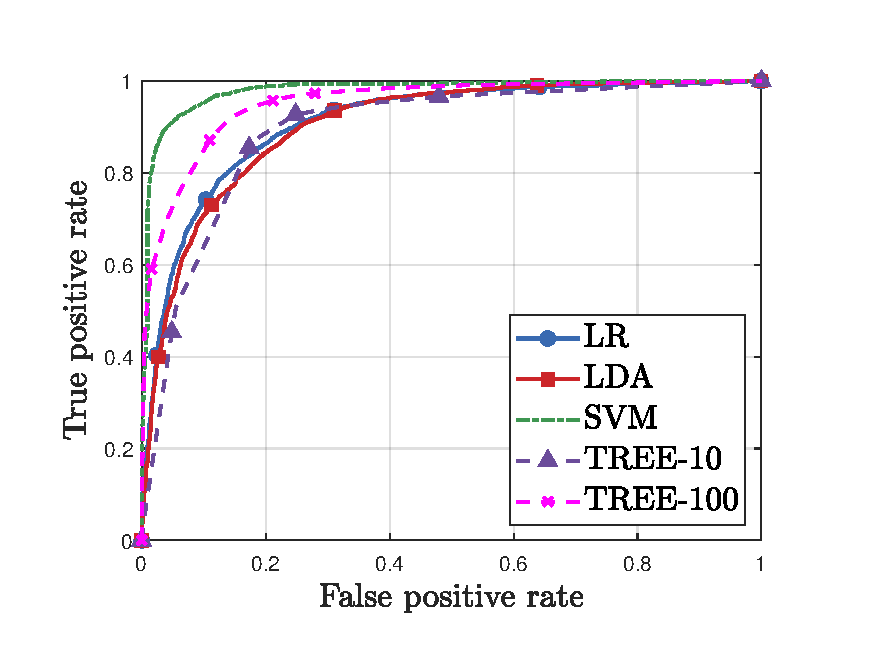
\includegraphics[width=0.5\textwidth]{../../code/hw3/matlab/figures/ROC.pdf}}
  \caption{ROC plot to illustrate the ability of each binary classifier system as its discrimination threshold is varied.}
  \label{fig:ROC}
\end{figure}

From the Table~\ref{tab:results}, we may assess the time necessary for train and test each model. SVM presents the best CV accurracy, howevere it presents the worst train duration, four times the second longest model train. The others methods present similar CV accuracy perfomance, while their cost is way less than SVM, except for KNN, with $K=1$. 
Among the presented methods, the test time is very short, less than a second.

The model choice depends on the scenario, the Decision Tree with ten nodes presents a very CV accuracy, similar to SVM, and it last less than a second to train. Hence, the advantages presented allow us to point out the decision tree as the best model.

\section{Discussion}


\section{Conclusion}
Dentre os resultados obtidos o não foram constatadas grandiosas diferenças dentre os resultados dos modelos, isso favorece a utilização de modelos mais simples e de menor custo computacional, em detrimento da pouca melhora da predição com o aumento do custo. Portanto ao menos que de fato haja uma necessidade em obter o melhor resultado possível, a solução com melhor custo-benefício foi a regressão linear simples, visto que é pouco custosa e obteve resultados não muito inferiores aos seus correntes, mas caso o custo computacional não precise ser considerado, o melhor modelo para o conjunto de dados fornecido é o de regressão ``ridge'', pois esse foi o que obteve os melhores resultados tanto na validação quanto no conjunto de teste.


\section{Further Work}


\bibliographystyle{ieeetran}
\bibliography{refs}

\end{document}